\documentclass[11pt]{article}
\usepackage[margin=0.9in]{geometry}
\usepackage{graphicx}
\usepackage{hyperref}
\usepackage{float}
\usepackage{booktabs}
\usepackage{colortbl}
\usepackage{amsmath}

\title{Threshold Experiment Report — Unknown Species Detection}
\author{Myco Fungi Project}
\date{April 2, 2026}

\begin{document}
\maketitle

% ============================
\section{Objective}
% ============================
Detect unknown fungal species at query time using a threshold on KNN retrieval
similarity scores, without any fine-tuned classifier.
The system must \textbf{accept} known species (5 \textit{Penicillium} target species)
and \textbf{reject} unknown species (all other species).
The optimisation target is \textbf{F1 score} on the positive (known) class.

% ============================
\section{Datasets}
% ============================
\subsection{Database (Qdrant collection)}
\begin{itemize}
  \item \textbf{Collection}: \texttt{myco\_fungi\_features\_full\_finetuned}
  \item \textbf{Extractor}: EfficientNetB1\_finetuned (1280-d)
  \item \textbf{Growth media}: MEA, CYA, DG18, CREA, YES, OA (all environments)
\end{itemize}

\subsection{Query / Test set}
\begin{itemize}
  \item \textbf{Source}: \texttt{results/threshold/diverse\_retrieval\_results.csv}
  \item \textbf{Total samples}: 861
  \item \textbf{Known species} ($is\_known=1$): 210
  \item \textbf{Unknown species} ($is\_known=0$): 651
  \item \textbf{Retrieval}: $k=11$, E1 (same growth medium), weighted aggregation
  \item \textbf{Train/test split}: One strain per species held out; all other strains
        of the same species remain in the database.
\end{itemize}

\subsection{Known species}
\textit{Penicillium citreonigrum}, \textit{P. commune}, \textit{P. crustosum},
\textit{P. expansum}, \textit{P. chrysogenum}

% ============================
\section{Query Construction}
% ============================
At query time each plate image passes through:

\begin{enumerate}
  \item \textbf{Segment} — KMeans isolates the petri-dish region; 1--3 colony
        segments are extracted per plate.
  \item \textbf{Feature extraction} — Each segment is passed through
        EfficientNetB1\_finetuned to produce a 1280-d embedding.
  \item \textbf{KNN retrieval} — Qdrant KNN ($k=11$) with \texttt{env\_strategy=E1}
        (only neighbours from the same growth medium) using named vector
        \texttt{EfficientNetB1\_finetuned}.
  \item \textbf{Sibling filtering} — Same-plate neighbours are excluded.
  \item \textbf{Score extraction} — Top-5 neighbour cosine similarities are recorded
        as $s_0 \dots s_4$ alongside each neighbour's species label.
\end{enumerate}

The retrieval CSV records these five scores per query plus the ground-truth
$is\_known$ flag (1 if the query's species is in the target set, 0 otherwise).

% ============================
\section{Why Autoresearch?}
% ============================
Manual search over formula $\times$ threshold combinations is intractable:
\begin{itemize}
  \item The formula space is open-ended: ratio chains, gap functions,
        polynomial transforms, weighted sums, entropy variants, etc.
  \item Three threshold algorithms ($\texttt{f1\_grid}$, $\texttt{roc\_opt}$, $\texttt{otsu}$)
        each favour different formulas.
  \item There are strong interaction effects: the best formula for one algorithm
        is not necessarily best for another.
\end{itemize}
The autoresearch pattern addresses this with: structured logging of every
(formula, algorithm, threshold) triple to \texttt{all\_experiments.csv};
staircase visualisation (grey = discarded, green = new best); active reading of
the log before each run to avoid repeating failures; and small focused scripts
(100--800 formulas per attempt) to keep experiments interpretable.

% ============================
\section{Methodology Diagram}
% ============================
\begin{figure}[H]
\centering
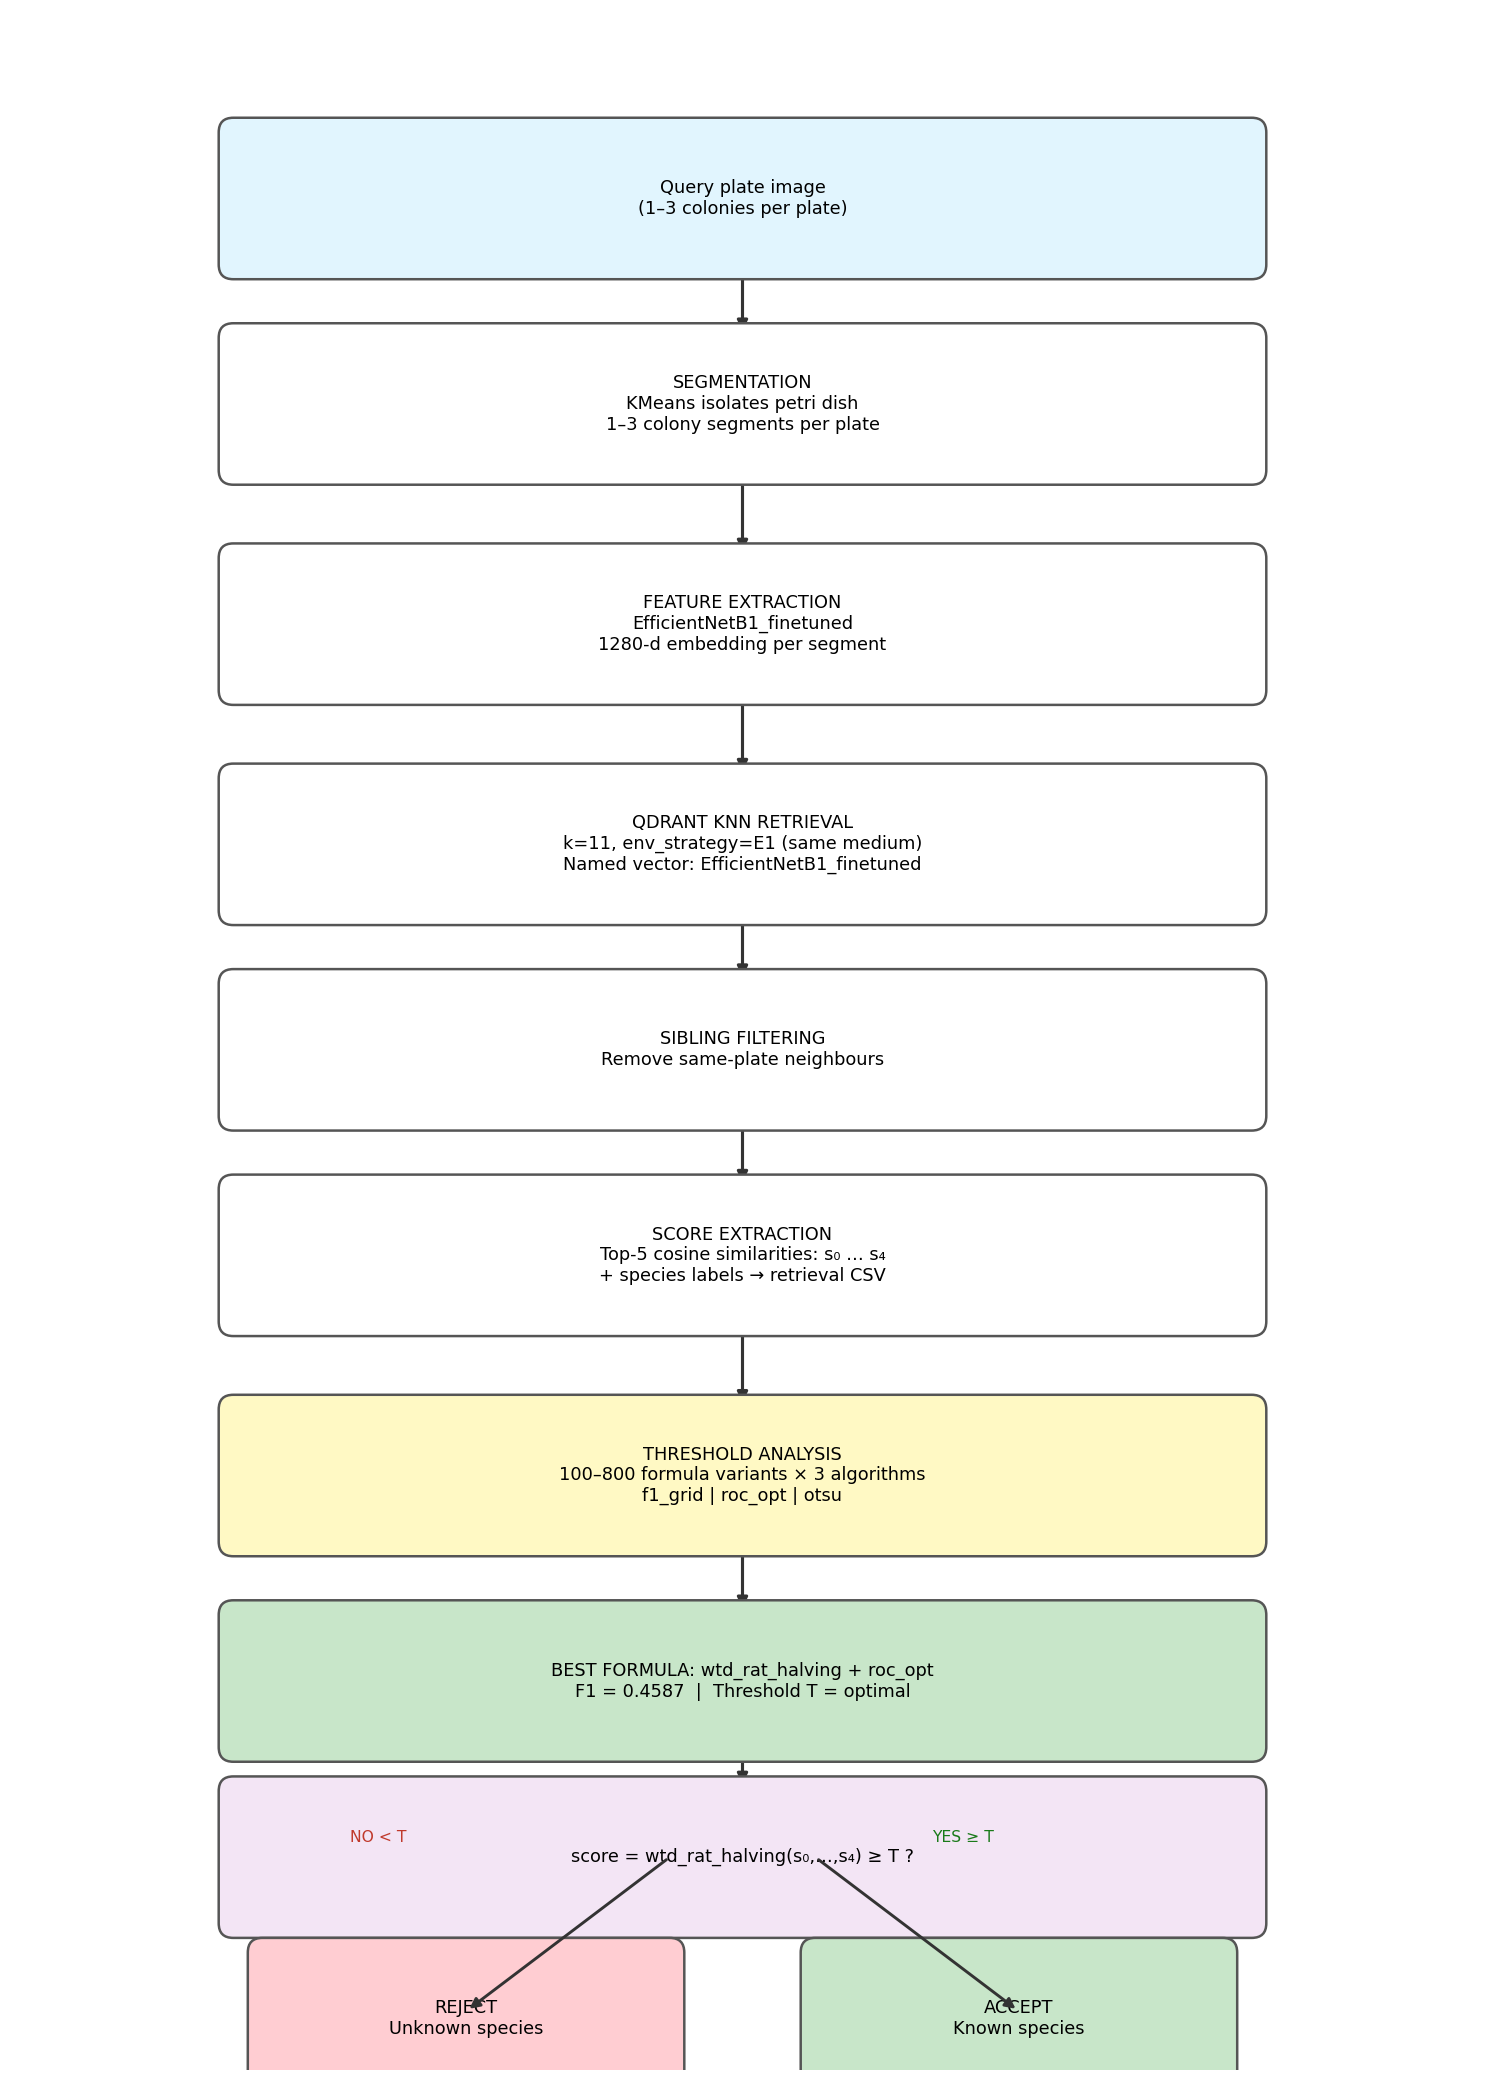
\includegraphics[width=0.72\textwidth]{images/methodology_diagram.png}
\caption{Retrieval pipeline (top) producing neighbour scores $s_0\ldots s_4$,
         followed by threshold analysis (middle) evaluating hundreds of
         formula $\times$ algorithm combinations, finally producing a
         binary known/unknown classifier (bottom).}
\label{fig:methodology}
\end{figure}

% ============================
\section{Experiment History}
% ============================
\begin{table}[H]
\centering
\begin{tabular}{ccllcr}
\toprule
Att. & \multicolumn{1}{c}{Date} & \multicolumn{1}{c}{Experiments} &
  Best Formula & \multicolumn{1}{c}{F1} & \multicolumn{1}{c}{Notes} \\
\midrule
1 & 2026-04-01 & 25 & abs\_gap\_f1\_grid & 0.0900 & baseline \\
2 & 2026-04-01 & 125 & geom\_mean\_top3\_roc\_opt & 0.1639 & +0.074 \\
3 & 2026-04-01 & 571 & geom\_mean\_top3\_roc\_opt & 0.1639 & no change \\
4 & 2026-04-01 & $\sim$500 & ratio\_s0s2\_roc\_opt & 0.4475 & labels fixed \\
5 & 2026-04-01 & 810 & rat01\_p\_rat12\_roc\_opt & 0.4536 & +0.006 \\
6 & 2026-04-02 & 306 & wtd\_rat\_halving\_roc\_opt & \textbf{0.4587} & +0.005 \\
\bottomrule
\end{tabular}
\caption{Autoresearch history. Key turning point: Attempt 4 corrected the
         $is\_known$ label encoding, jumping F1 from $\sim$0.09 to $\sim$0.45.}
\end{table}

% ============================
\section{Best Strategies (Top-5)}
% ============================
\begin{table}[H]
\centering
\begin{tabular}{llccccccc}
\toprule
Rank & Formula & Algo. & \multicolumn{1}{c}{F1} & P & R & Spec &
  \multicolumn{1}{c}{TP} & \multicolumn{1}{c}{FP} \\
\midrule
1 & wtd\_rat\_halving & roc\_opt & \textbf{0.4587} & 0.319 & 0.819 & 0.435 &
  172 & 368 \\
2 & spread\_012\_ov\_s0 & f1\_grid & 0.4579 & 0.322 & 0.791 & 0.464 &
  166 & 349 \\
3 & rat01\_p\_rat12\_m\_rat23 & f1\_grid & 0.4533 & 0.315 & 0.810 & 0.432 &
  170 & 370 \\
4 & wtd\_rat\_halving & f1\_grid & 0.4574 & 0.314 & 0.843 & 0.406 &
  177 & 387 \\
5 & rat01\_p\_rat12\_m\_rat23 & roc\_opt & 0.4536 & 0.318 & 0.791 & 0.453 &
  166 & 356 \\
\bottomrule
\end{tabular}
\caption{Top-5 strategies across all 2362 total experiments.
         The current best \texttt{wtd\_rat\_halving} extends the consecutive
         ratio idea across all 4 neighbour pairs with halving-decay weights.}
\end{table}

% ============================
\section{Confusion Matrices}
% ============================
The three key strategies are visualised below.

\begin{figure}[H]
\centering
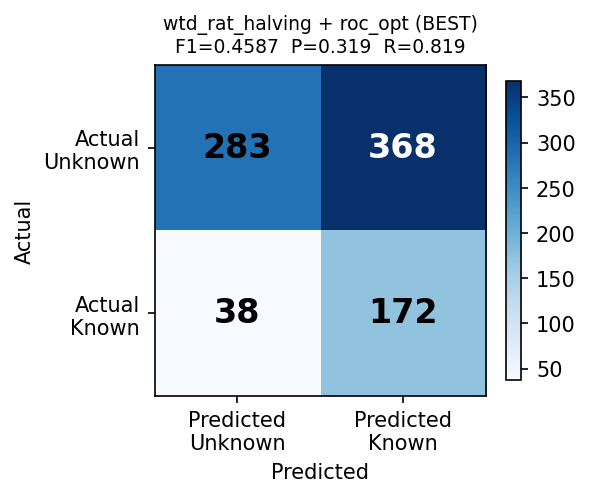
\includegraphics[width=0.32\textwidth]{images/cm_wtd_rat_halving_roc_opt.png}
\hfill
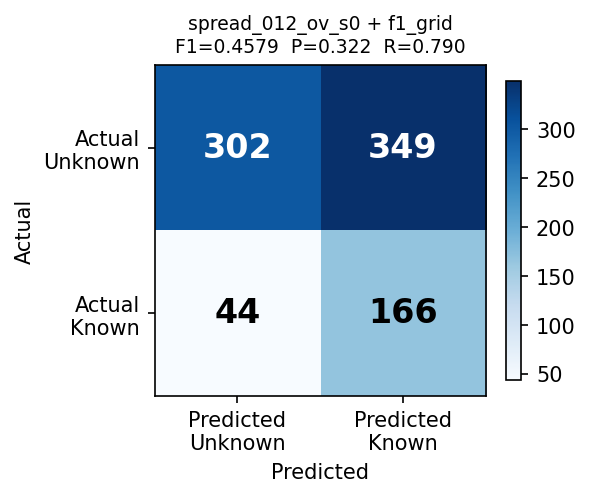
\includegraphics[width=0.32\textwidth]{images/cm_spread_012_ov_s0_f1_grid.png}
\hfill
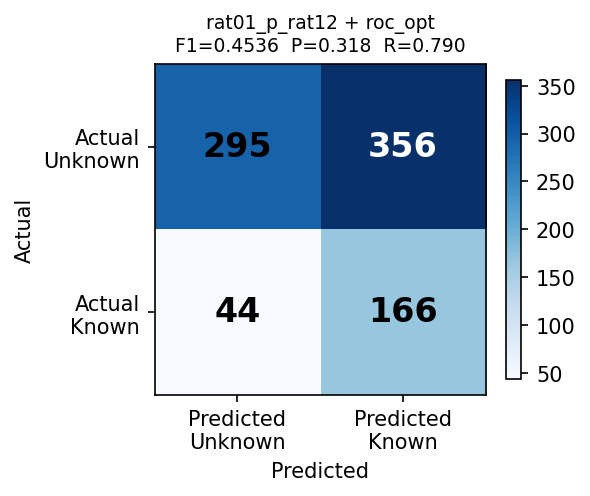
\includegraphics[width=0.32\textwidth]{images/cm_rat01_p_rat12_roc_opt.png}
\\[4pt]
{\small Left: wtd\_rat\_halving + roc\_opt (overall best, F1=0.4587).\\
 Centre: spread\_012\_ov\_s0 + f1\_grid (best f1\_grid, F1=0.4579).\\
 Right: rat01\_p\_rat12 + roc\_opt (previous best, F1=0.4536).}
\caption{Confusion matrices for the three key strategies.}
\label{fig:confusion}
\end{figure}

% ============================
\section{Formula Family Analysis}
% ============================
\subsection{Ratio-chain family}
Consecutive ratios $s_i/s_{i+1}$ capture how much the top match dominates
its immediate neighbour --- a proxy for retrieval confidence.

\medskip
\noindent
Extended chains with decay consistently outperform the 2-term sum:

\begin{itemize}
  \item \texttt{wtd\_rat\_halving} $= 1.0\cdot(s_0/s_1) + 0.5\cdot(s_1/s_2)
        + 0.25\cdot(s_2/s_3) + 0.125\cdot(s_3/s_4)$: F1=0.4587
  \item \texttt{wtd\_rat\_015} (base-1.5 decay, 4-term): F1=0.4530
  \item \texttt{rat01\_p\_rat12} (2-term sum, previous best): F1=0.4536
  \item \texttt{rat012\_sum} (3-term sum): F1=0.4512
\end{itemize}

Extending to all 4 consecutive pairs with halving decay yields the best result,
suggesting that diminishing contributions from distant ranks carry useful signal.

\subsection{Spread / diversity family}
Spread metrics (coefficient of variation of top-$k$ scores) quantify retrieval
ambiguity:

\begin{itemize}
  \item \texttt{spread\_012\_ov\_s0} $= \frac{\text{std}(s_{0:3})}{\text{mean}(s_{0:3})} / s_0$: F1=0.4579
  \item \texttt{gnorm02\_sq} $(s_0-s_2)^2/(s_0+s_2)^2$: F1=0.4475
\end{itemize}

High spread indicates a clear dominant match; low spread indicates ambiguous
retrieval. Normalising by $s_0$ removes the absolute scale, improving
discrimination.

% ============================
\section{Key Insights}
% ============================
\begin{enumerate}
  \item \textbf{Retrieval confidence is separable}: The gap/ratio between top
        neighbour scores is far more discriminative than raw $s_0$ alone.
        F1 for $s_0$ alone $\approx$ 0.08; best ratio-chain formulas reach
        F1 $\approx$ 0.46.
  \item \textbf{Chain length and decay matter}: Extending consecutive ratios
        beyond $s_0/s_1+s_1/s_2$ to all 4 pairs with halving-decay weights
        gives a small but consistent improvement.
  \item \texttt{roc\_opt} outperforms \texttt{f1\_grid} on most top formulas
        by balancing sensitivity and specificity via Youden's $J$.
  \item \textbf{Precision ceiling}: Best precision $\approx$ 32\%; the main
        failure mode is confusing unknown species with known ones (high FP).
  \item \textbf{Recall is strong}: Best recall $\approx$ 84\%. The bottleneck
        is false positives, not false negatives.
\end{enumerate}

% ============================
\section{Future Directions}
% ============================
\begin{itemize}
  \item Train a separate binary classifier (logistic regression / SVM) on
        top of retrieval features rather than a single scalar threshold.
  \item Ensemble multiple extractors (ResNet50\_finetuned + MobileNetV2\_finetuned)
        before applying the threshold.
  \item Use top-1 species softmax confidence or temperature-scaled scores as
        additional signal.
  \item Investigate whether the FP unknown species share morphological
        similarity to the known set (e.g. shared colony texture / colour).
\end{itemize}

% ============================
\section{Autoresearch Staircase}
% ============================
\begin{figure}[H]
\centering
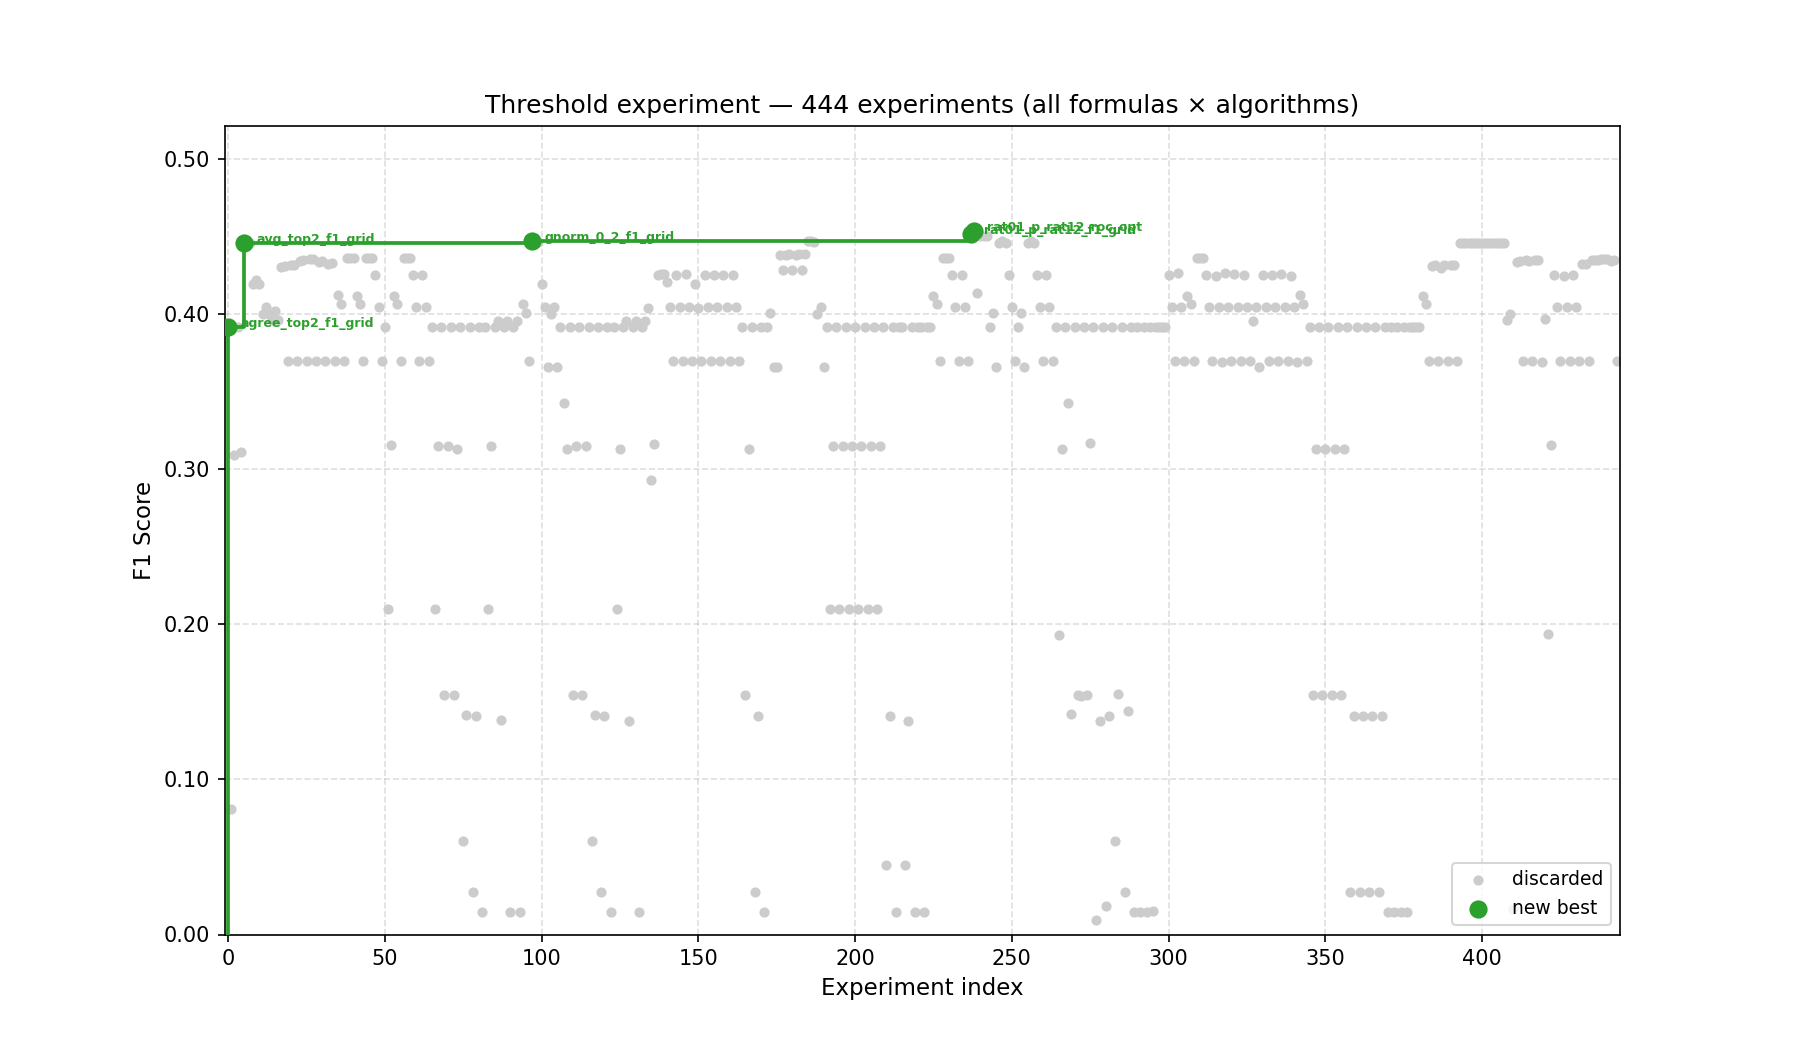
\includegraphics[width=\textwidth]{images/staircase.png}
\caption{Autoresearch staircase chart. Each dot is one individual
         formula $\times$ algorithm experiment. Gray = discarded (F1 $\le$ running best);
         green = new running best. The step-up pattern shows improvement over attempts.}
\label{fig:staircase}
\end{figure}

% ============================
\section{Supporting Visualisations}
% ============================
\begin{figure}[H]
\centering
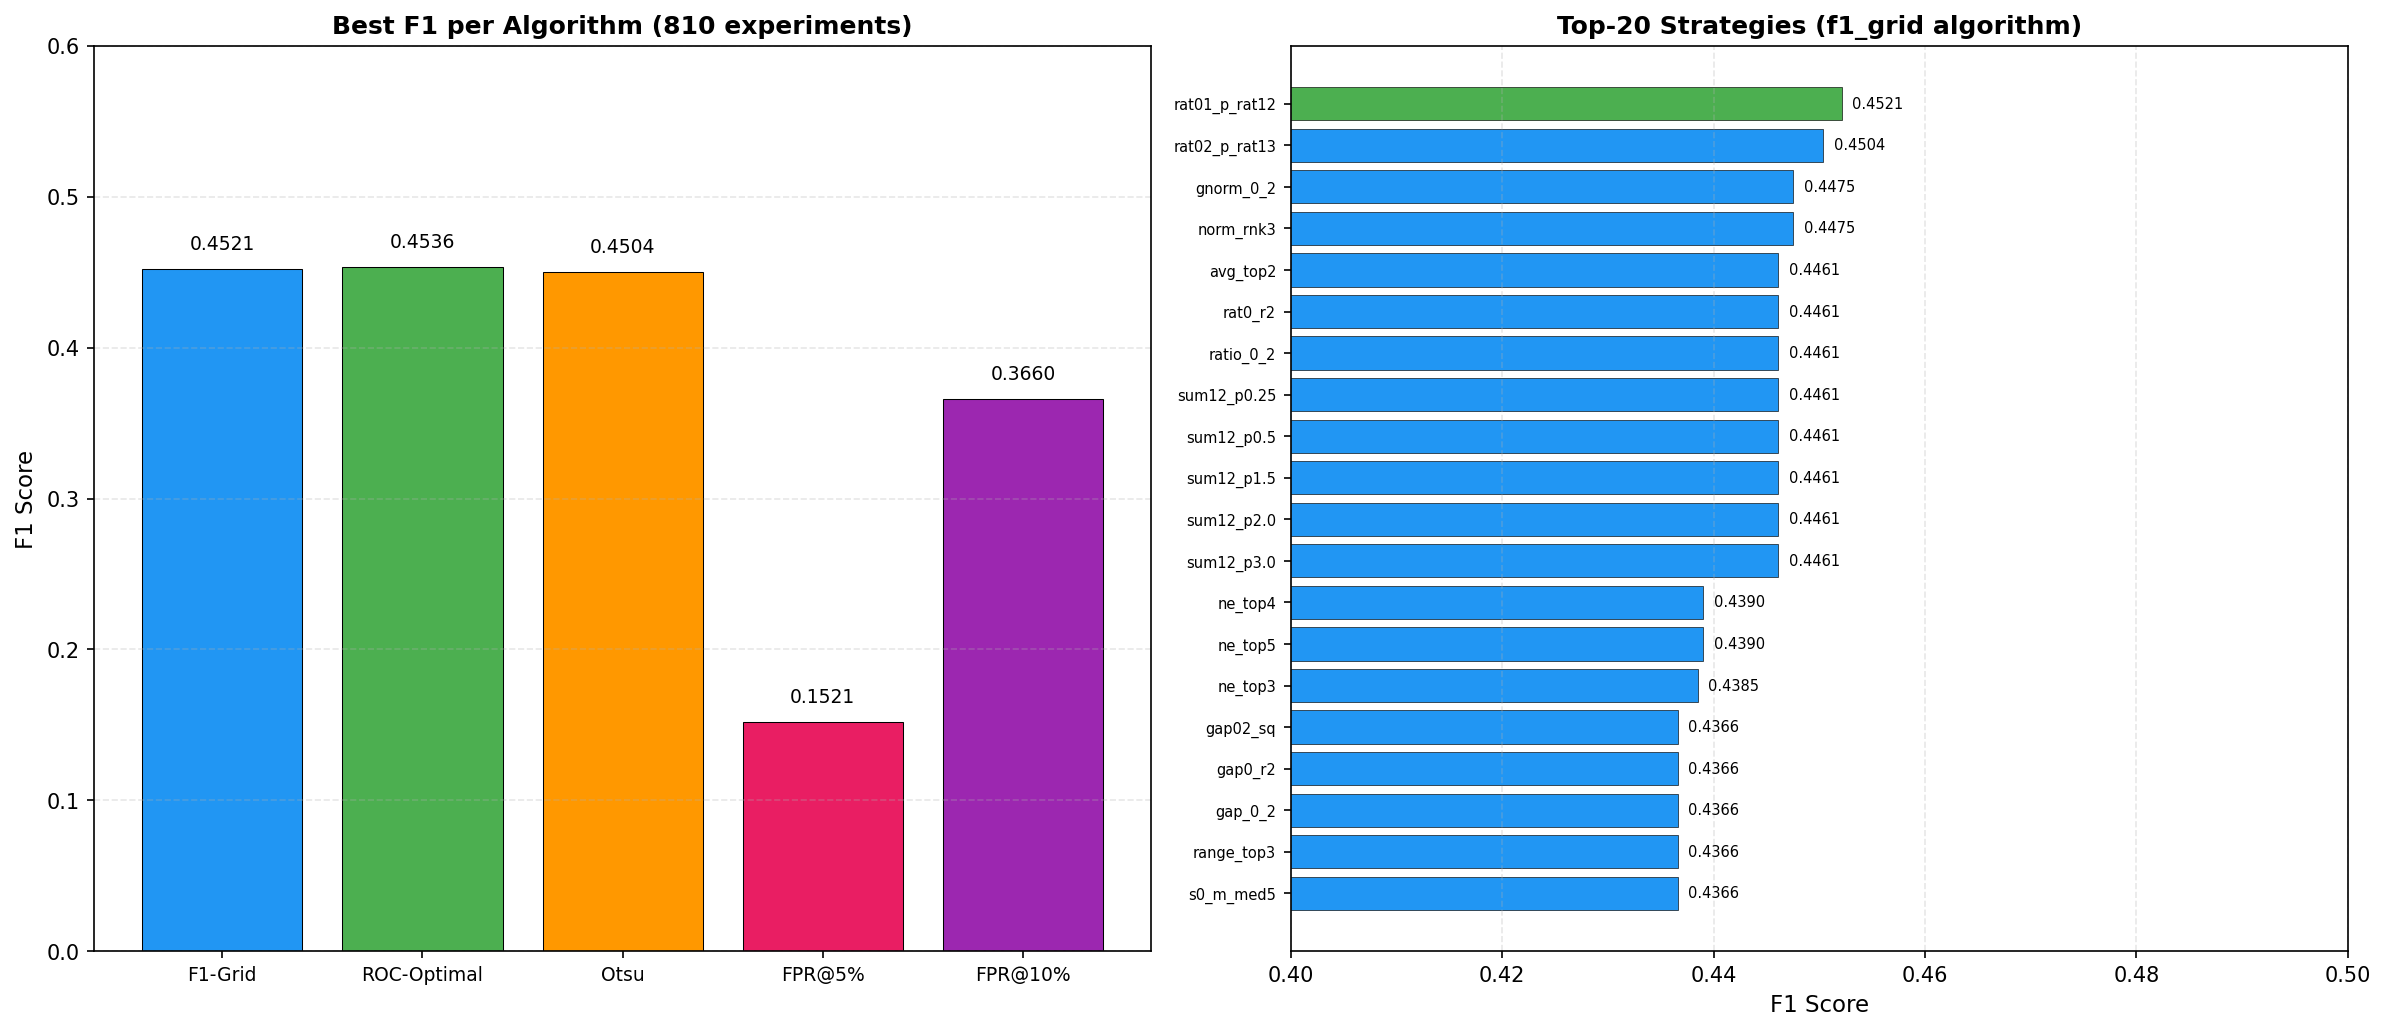
\includegraphics[width=0.48\textwidth]{images/top_strategies_summary.png}
\hfill
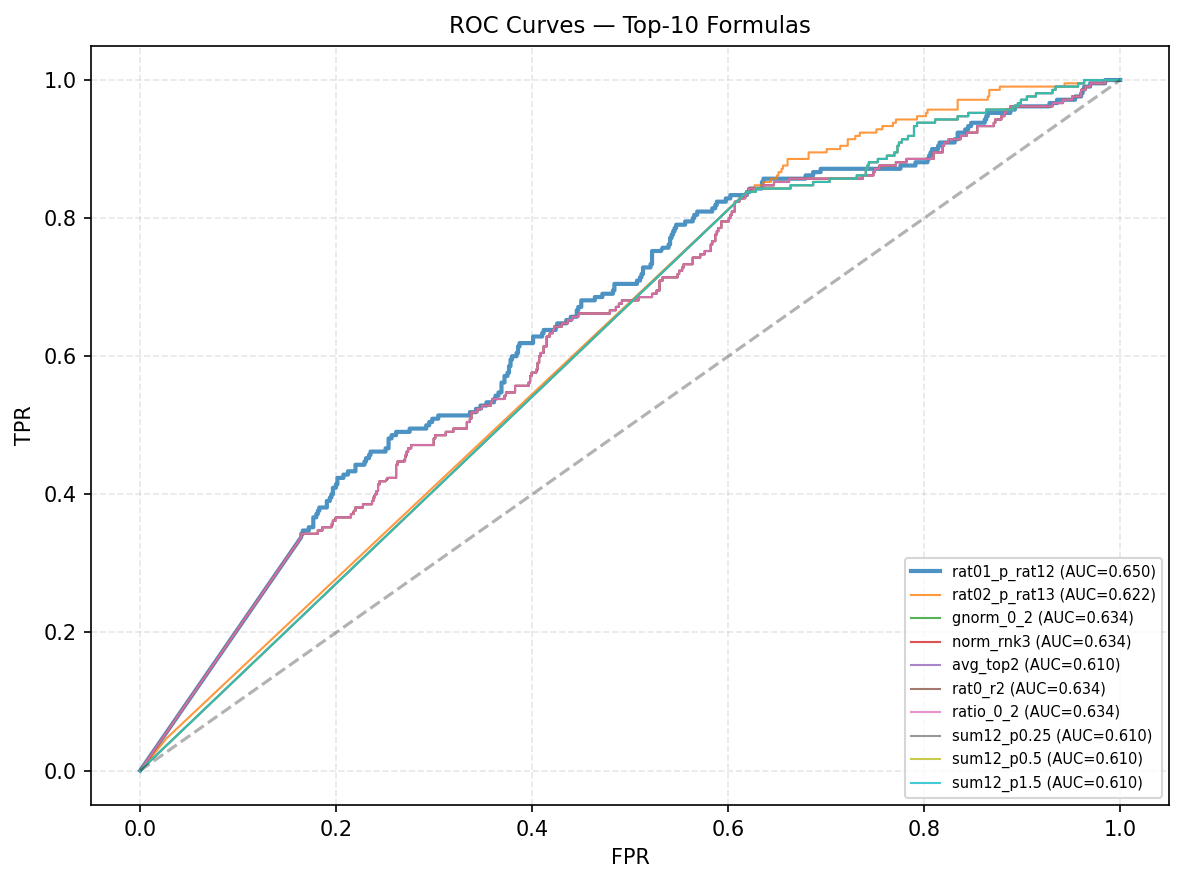
\includegraphics[width=0.48\textwidth]{images/roc_curves.png}
\caption{Left: Top-20 strategy F1 scores across all attempts.
         Right: ROC curves for the three best strategies.}
\label{fig:extras}
\end{figure}

\begin{figure}[H]
\centering
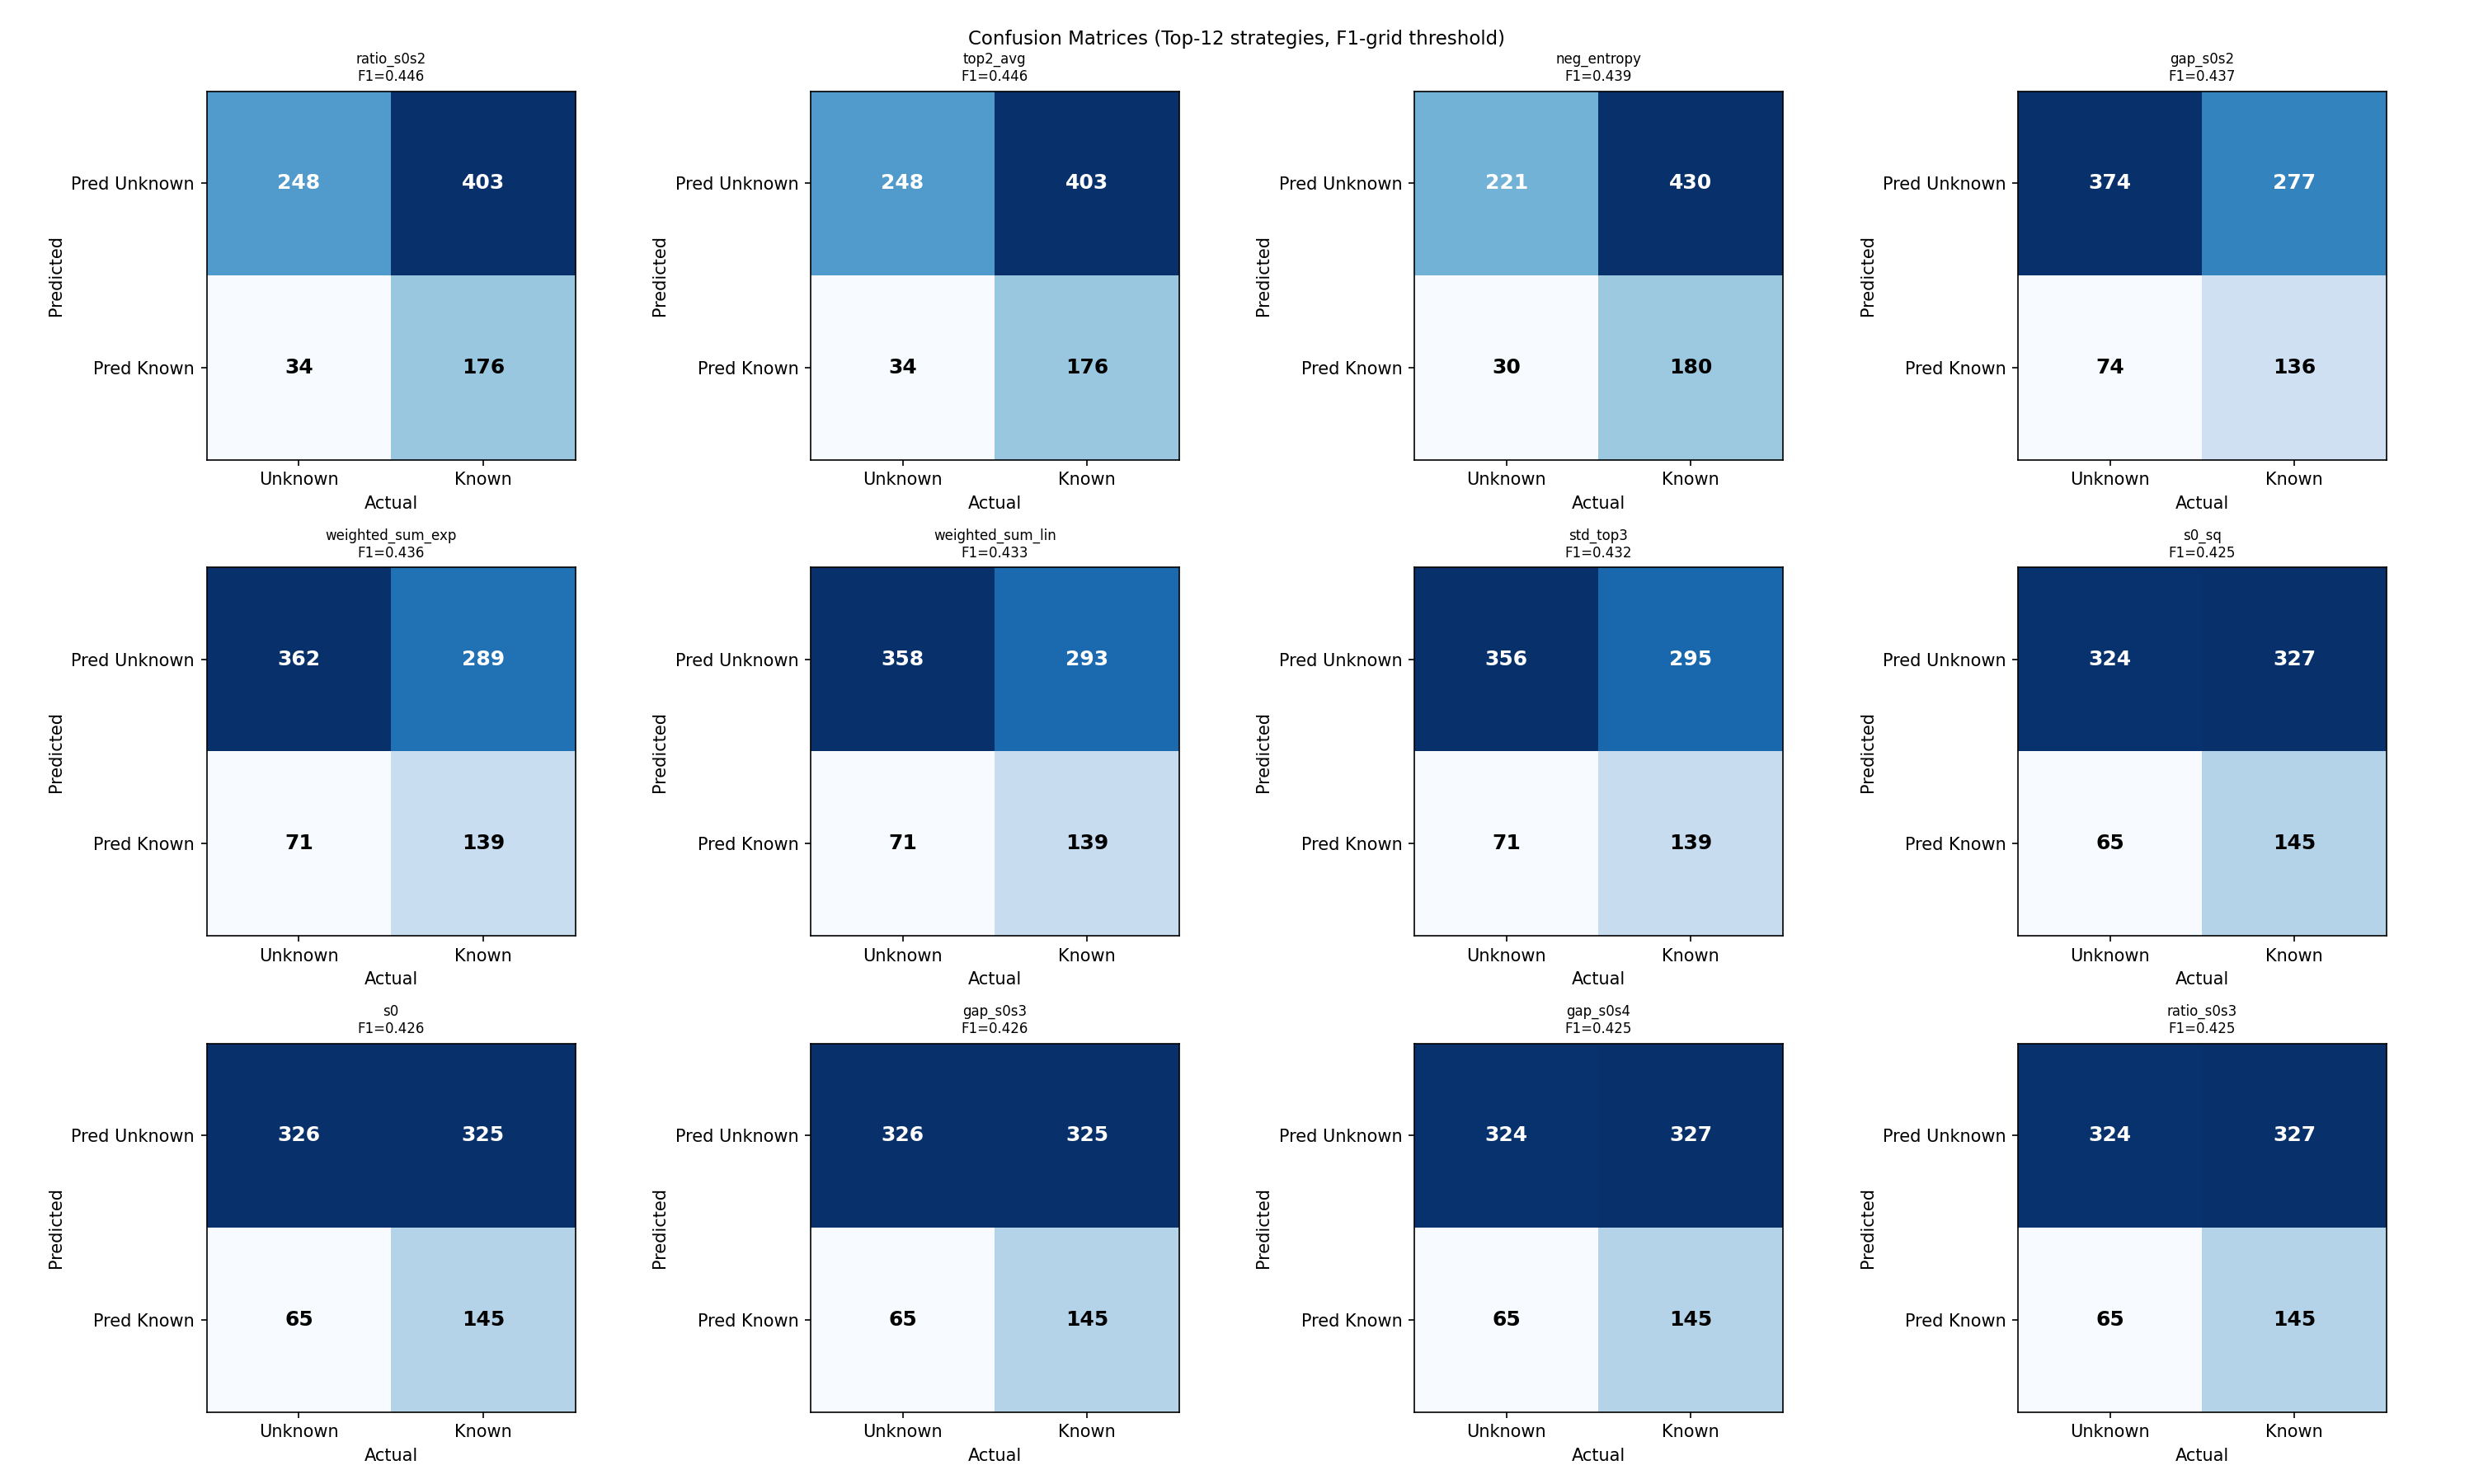
\includegraphics[width=\textwidth]{images/confusion_matrices_full.png}
\caption{Confusion matrices across all top strategies in the final attempt.}
\label{fig:cm_full}
\end{figure}

\end{document}
